
In the previous chapter we explained how the dynamics of brane stacks, in particular D3-branes in type IIB, are described by gauge field theory on their worldvolumes. It's however important to note that parallel to this open string picture of the brane stack system there is also a dual description in terms of the curved spacetimes generated by their mass and Ramond-Ramond charge. Insisting these two viewpoints are equivalent, one is able to deduce an exact correspondence between the gauge theory and string theory on a specific background geometry.

This kind of duality is exotic as it connects a local field theory in four dimensions with a ten-dimensional string (and so, inherently gravitational) theory through a perfect mapping. It is reasonable in fact to identify the spacetime of the field theory with the conformal boundary of the higher-dimensional dual gravitational background (the bulk), for reasons we will clarify - so that in more colloquial language the dynamics in the bulk are ``encoded'' in the screen at infinity, hence the adjective ``holographic'' for this sort of correspondences.

Explicit holographic correspondences are not only interesting by themselves as elegant structures; they are also extremely practical tools for studying the theories involved on both sides. It is certainly very attractive for the purpose of quantum gravity or the definition of string theory - non-local theories without action functionals - if these situations happen to be equivalent to a local quantum field theory.

%For example: if a gravitational, and therefore stringy, theory on a certain background is dual to a 4D field theory, entropy will scale as the boundary (hyper-)area, and not like the bulk volume, as we'd expect if the gravitational side were a local field theory. The nonlocality

However in this work our interest will be focused on the opposite direction, investigating the dynamics of the field theory by exploiting the dual gravitational system. The power of holographic dualities lies in the fact that they map the strongly-coupled regime for the field theory to the regime where the bulk dynamics can be approximated by supergravity. The traditionally untreatable strong coupling region for some gauge QFTs in four dimensions can then be probed by studying the relatively tamer dynamics of a smooth dual spacetime.



\section{Maldacena duality}

We introduce now the simplest and most celebrated example of holographic correspondence. Consider the IIB supergravity solution for the warped spacetime created by a system of D3-branes in a background $\mathbb{R}^{1,9}$. We specialize the solution of section \ref{sec:pbranes} to $p=3$:

\begin{align}
	ds^2 = H^{-1/2} dx_\mu dx^\mu + H^{1/2} (dr^2 + r^2 d\Omega^2_5)\label{black3metric}\\	
	e^\Phi = \mathrm{const} =: g_s \\
	F_5 = dH^{-1} \wedge dx^0 \wedge dx^1 \wedge dx^2 \wedge dx^3
\end{align}

\begin{equation}
	H(r) = 1 + \left( \frac{R}{r} \right)^4
	\label{}
\end{equation}

where $x^\mu$, $\mu = 0,\ldots,3$ are coordinates parallel to the brane stack and $d\Omega_5$ is the standard metric on $\mathbb{S}^5$.\\

The curvature radius $R$ is given by

\begin{equation}
	R^4 = 4\pi g_s N \alpha'^2 = g_{YM}^2 N \alpha'^2
	\label{}
\end{equation}

where $N$ is the number of D3-branes in the stack.\\

We note an important peculiarity of this metric as opposed to analogous solution for the Dp-brane with $p\neq 3$: there exists a horizon at $r=0$, but this horizon is an infinite distance away, namely

\begin{equation}
	\int_\varepsilon^{r'} \left( 1 + \left( R/r \right)^4 \right)^{1/4} dr \sim -\ln\varepsilon
	\label{}
\end{equation}

therefore the ``near-horizon'' ($r<<R$) geometry takes the form of an infinitely long ``throat''. This should be compared, just to make an example, to the Schwarzschild solution where the horizon is at a finite distance from any given point in the exterior. This throat feature will play a crucial role for the AdS/CFT correspondence, as will be seen shortly.\\

This system (IIB string theory on the metric \ref{black3metric}) must then be equivalent to the stack of D3-branes in the background Minkowski, taking into account both open and closed string interactions. The action is schematically:

\begin{equation}
	S = \frac{1}{g_s} \int d^4 x F^2 + \frac{1}{\alpha'^4} \int d^{10}x \sqrt{g} R e^{-2\phi} + O(\alpha') + \dots
\end{equation}

(since, we recall, $g_{YM}^2 \sim g_s$). The first two terms are respectively the actions for SYM and free IIB SUGRA in the Minkowski background; the following terms, with higher powers of $\alpha'$, establish the coupling between these two systems. It's clear that in the limit $\alpha' \rightarrow 0$ the free SUGRA part decouples from the SYM.\\

We repeat this decoupling limit for the black 3-brane metric. If $\alpha' \rightarrow 0$, so does $R$, and effectively the metric seems to converge to flat spacetime. We have however to take into consideration the throat described before. The throat shrinks as $R^2 \sim \alpha' \rightarrow 0$; to maintain focus on it as we lower the Regge slope we need to rescale our $r$ coordinate. We can introduce $\phi = r/\alpha'$ and keep $\phi$ fixed as $\alpha'$ goes to zero. With this choice the metric actually reduces to

\begin{equation}
	ds^2 = \alpha' \left( \frac{\phi^2 }{R^2}dx^\mu dx_\mu + \frac{R^2}{\phi^2} d\phi^2 + R^2 d\Omega_5^2 \right)
	\label{}
\end{equation}

which is actually the metric for the product space $AdS_5 \times \mathbb{S}^5$. Therefore under $\alpha' \rightarrow 0$ also on the black brane side we have a decoupling of two systems, IIB on Minkowski, and IIB on the near-horizon geometry.\\

The essential point is that if the two pictures are to be equivalent, and so SYM4 plus decoupled IIB on Minkowski is to be equal to IIB on $AdS_5 \times \mathbb{S}^5$ plus decoupled IIB on Minkowski, then intuitively one expects to be able to ``subtract off'' the decoupled theory from both sides and obtain an equivalence between the gauge theory and the gravitational theory on $AdS_5 \times \mathbb{S}^5$. This intuition turns out to be correct, though the details of this equivalence have to be specified. In any case, this is the simplest (and most famous) case of an AdS/CFT correspondence.\\

We clarify that the decoupling / near-horizon limit we implemented must be generalized carefully to the case of non-coincident branes, since we will be particularly interested in those kind of configurations. If two branes are a distance $\Delta r$ apart, there will be massive Higgses from open strings stretching between them, with masses of the order of the string tension times the distance: $m \sim \Delta r / \alpha'$. We would like to keep this masses constant. The obvious choice is then to rescale the brane $r$ positions as $\phi_i = r_i / \alpha'$ and keep those constant as we zoom in. This is what we will refer to as the near-horizon limit in the general case and the resulting geometry as the near-horizon warped geometry.\\

The relevance of the large $N$ limit to the correspondence is evident when it's translated to a limit in the AdS side. Keeping $\lambda = g_{YM}^2 N$ constant and sending $N \gg 1$, considering that

\begin{equation}
	4\pi g_s = \frac{\lambda}{N}
	\label{}
\end{equation}

is equivalent to having $g_s \ll 1$. Weak string coupling amounts to a suppression of string loops and effectiveness of the perturbative expansion. A more surprising conclusion concerns however the limit of large 't Hooft coupling $\lambda \gg 1$, since

\begin{equation}
	\frac{R^2}{\alpha'} = \sqrt \lambda
	\label{}
\end{equation}

so that large coupling means a large $\mathbb{S}^5$ radius. This implies two desirable suppressions: of the massive Kaluza-Klein-like modes wrapping around the $\mathbb{S}^5$, and of terms with more than two derivatives in the effective action. In essence, the dual physics is well described by IIB supergravity, a field theory, instead of full string theory.\\

Combining both results, a large $N$, strong-coupling gauge theory will be dual to weakly-coupled supergravity. The strong/weak interchange is what earns the correspondence the title of ``duality''. In the next section the connotation of ``holographic'' will also be justified.

\section{Large $N$ limit}

It was just seen how the weak-coupling regime for the string theory maps to a ``large N'' limit on the gauge theory side. How this limit is understood has to be explained more carefully.

Consider a gauge theory of the type considered in chapter \ref{chap:cones}, with an $SU(N)^g$ gauge group. The bosonic part of the Lagrangian is

\begin{equation}
\mathcal{L} = \Tr \left(F^2\right) + \ldots 
\end{equation}

with $F_{\mu\nu} = \partial_\mu A_\nu - \partial_\nu A_\mu + i g_{YM} [A_\mu,A_\nu]$ and $\ldots$ can include fields in adjoint and bifundamental representations\footnote{The following construction can be extended to include particles in the (anti-)fundamental, but the details are different and this case is not relevant to our interests.}, and all irreps obtainable by tensoring these. Ultimately, all fields will be representable as objects with a certain number of colour indices, at most related by symmetries in those indices.

We can modify the standard Feynman prescription for pictorially representing amplitudes to get a "double line" or "ribbon" representation in which each colour index is carried by a line. For example, the gluon self energy diagram becomes as such:

\begin{center}
\def\svgwidth{200pt}
\input{images/strips.pdf_tex}
%\caption{}
\end{center}

colour indices $i$, $\bar i$, $j$, $\bar j = 1 , \ldots , N$ are fixed, while $k$ must be summed over. The amplitude has two three-gluon vertices, each carrying a factor of $g_{YM}^2$, for an overall factor of $g_{YM}^2 N$.

It iss easy to convince oneself that as long as we restrict to planar diagrams, that is diagrams that can be drawn on the plane (or more precisely the sphere), adding one strip will always introduce exactly one additional loop and two additional vertices, again carrying a factor of $g_{YM}^2 N$. The combination $\lambda := g_{YM}^2 N$ is the 't Hooft coupling, and is better suited to represent the strength of the gauge interaction than $g_{YM}$ if we are to modify the number of colours.

Then, the 't Hooft large $N$ limit is defined as:

\begin{equation}
N \rightarrow \infty, \quad \mathrm{but \; keeping } \; \lambda \; \mathrm{fixed.}
\end{equation}

Equivalently, keeping $\lambda$ constant and sending $g_{YM} \rightarrow 0$.

A useful rescaling of the fields shifts all the $g_{YM}$ dependence of the Lagrangian to a factor in front:

\begin{equation} \label{rescaling} \mathcal{L} = \frac{1}{g_{YM}^2} \left( \Tr F^2 + \ldots \right) \end{equation}

so that now all types of vertices bring $g_{YM}^2 = \lambda/N$ and propagators bring $1/g_{YM}^2 = N/\lambda$.\\

We extend to nonplanar graphs by noting these can always be drawn on some Riemann surface of genus $h$, and, since they induce triangular tilings of said surface, the famous formula for the Euler characteristic holds:

\begin{equation}
F - V + E = \chi = 2 - 2h 
\end{equation}

$F$, $V$, $E$ being the number of faces, vertices, edges respectively. Now each face (loop) carries a factor of $N$, each vertex a factor of $\lambda/N$, and each edge $N/\lambda$, so that the total contribution is

\begin{equation}
\lambda^{E-V} N^{F-V+E} = \lambda^{E-V} N^{2-2g} 
\end{equation}

so that at fixed $\lambda$, an expansion in $N$ (or better $1/N$) is a genus expansion reminiscent of the loop expansion in perturbative string theory. This for example means that the free energy admits a power expansion in $1/N$:

\begin{equation}
F = \sum_{g=0}^\infty f_g(\lambda) N^{2-2g}\,.
\end{equation}

In conclusion, the 't Hooft limit results in suppression of the higher-genus contributions by powers of $N^{-2}$ with respect to the planar diagrams\footnote{One could be perplexed by the $N^2$ divergence of the genus zero contribution. This is not problematic however; it's an artifact of the rescaling \ref{rescaling} which makes the Lagrangian itself diverge as $g_{YM}^{-2} \Tr F^2 \sim N/\lambda \cdot N$, since the trace of a matrix in the adjoint scales as $N$.}, and is thus also known as the planar limit. It is remarkable that this genus expansion is reminiscent of the string genus expansion, and that their regimes of effectiveness in holographic dualities coincide.

\section{Features of AdS/CFT}

Having ascertained that a correspondence of some form exists, one would then seek a more precise description of how the mapping between the four-dimensional gauge theory (the boundary) and the supergravity side (the bulk) is structured. In general, one has what is called an operator-state correspondence: operators in the boundary are associated by a holographic dictionary to ``states'', or classical solutions in the bulk. More precisely, consider a 4D local operator field $\hat \phi(x)$. The generating functional for its correlation functions is given by coupling it to a current $h(x)$:

\begin{equation}
	e^{W[h]} = \frac{1}{Z_\text{CFT}}\int D\psi e^{i S_\text{CFT} + \int d^4 x h(x) \hat \phi(x)}
\end{equation}

then, the source $h(x)$ is viewed as the limit as $r \rightarrow \infty$ of a five dimensional field configuration $h_5(x,r)$, given by solving the equations of motion from $S_{AdS}$ with $h(x)$ as a boundary condition. The correspondence is between the ``off-shell'' boundary operator $\int d^4 x \hat \phi(x)$ and the ``on-shell'' bulk configuration $h_5(x,r)$ - or between the fields $\hat \phi(x)$ and $h_5$, and states that the generating functional above is equal to the bulk action computed on the specific classical solution $h(x,r)$:

\begin{equation}
	e^{W[h]} = \langle e^{-\int d^4 x h \hat \phi(x)} \rangle_\text{CFT} = e^{iS_{AdS}[h_5]}
	\label{}
\end{equation}

Therefore, correlation functions for the strongly-coupled CFT can be calculated entirely through the weakly-coupled, two-derivatives bulk action.\\

One may then wonder about the interpretation one should employ for the fifth extra dimension in the bulk from the CFT perspective. A tentative identification comes from the fact that the AdS metric is invariant under dilations

\begin{equation}
	x^\mu \rightarrow \lambda x^\mu, \quad \quad z \rightarrow \lambda z
	\label{}
\end{equation}

Since $1/z$ scales like an energy, it could be paired holographically with the boundary energy scale. This turns out to be correct in the sense of renormalization: probing AdS at large distances, closer to the boundary at infinity (as we did before by coupling $\hat\phi(x)$ with the value at infinity of a 5D field) coincides with probing the microscopical, UV theory. Moving inwards, operators at larger values of $z$ equate probing the theory at a lower energy scale $\mu \sim 1/z$, up until the horizon which is identified with the IR. The fifth dimension is to be roughly identified with the renormalization flow of the field theory.\\

Therefore it might be useful to think of the microscopic field theory with no degrees of freedom integrated out, the UV limit, as being somewhat literally located at the conformal boundary at infinity of the AdS dual. Hence the ``boundary''/``bulk'' terminology, and since all of the physics in the 5D gravitational theory are encoded in a codimension-1 ``screen'' at infinity, one speaks of holography, in analogy with the real-life technique of encoding three-dimensional objects in a two-dimensional hologram.\\

In light of the above energy-$r$ relationship, our pairing of field configurations $h_5(x,z)$ with boundary operators has to be corrected. If $h_5(x,z)$ is asymptotically constant as $z\rightarrow 0$ so that the limit $h_5 \rightarrow h$ is well-defined, it must be that the corresponding dual operator does not scale under dilations, so that its conformal dimension $\Delta = 0$. The extension to CFT operators with arbitrary scaling dimensions is then realized by adding the possibility of $h_5(x,z)$ diverging as a power of $z$ as

\begin{equation}
	h_5(x,z) \rightarrow z^\Delta h(x)
	\label{}
\end{equation}

so that $h(x)$ can then be coupled as source to an operator of conformal dimension $\Delta$. This in turn will induce a dependency of $\Delta$ on the mass of the dual bulk field. As an example, let's take a scalar field in $AdS_5$ minimally coupled to the graviton:

\begin{equation}
	S \propto d^4 x\, dz \, \sqrt g \left( g^{mn} \partial_m h_5 \partial_n h_5 + m^2 h_5^2 \right)
	\label{}
\end{equation}

so that the classical equation of motion is (ignoring $x$ dependency, since it does not affect this argument):

\begin{equation}
	\partial_z \left( z^{-3} \partial_z h_5 \right) = z^{-5} R^2 m^2 h_5
	\label{ }
\end{equation}

plugging in a power law $h_5 = h z^\Delta$ yields the conformal dimension-mass relation:

\begin{equation}
	\Delta (\Delta-4) = R^2 m^2
	\label{}
\end{equation}

\begin{figure}[h!]
\centering
% GNUPLOT: LaTeX picture with Postscript
\begingroup
  \makeatletter
  \providecommand\color[2][]{%
    \GenericError{(gnuplot) \space\space\space\@spaces}{%
      Package color not loaded in conjunction with
      terminal option `colourtext'%
    }{See the gnuplot documentation for explanation.%
    }{Either use 'blacktext' in gnuplot or load the package
      color.sty in LaTeX.}%
    \renewcommand\color[2][]{}%
  }%
  \providecommand\includegraphics[2][]{%
    \GenericError{(gnuplot) \space\space\space\@spaces}{%
      Package graphicx or graphics not loaded%
    }{See the gnuplot documentation for explanation.%
    }{The gnuplot epslatex terminal needs graphicx.sty or graphics.sty.}%
    \renewcommand\includegraphics[2][]{}%
  }%
  \providecommand\rotatebox[2]{#2}%
  \@ifundefined{ifGPcolor}{%
    \newif\ifGPcolor
    \GPcolorfalse
  }{}%
  \@ifundefined{ifGPblacktext}{%
    \newif\ifGPblacktext
    \GPblacktexttrue
  }{}%
  % define a \g@addto@macro without @ in the name:
  \let\gplgaddtomacro\g@addto@macro
  % define empty templates for all commands taking text:
  \gdef\gplbacktext{}%
  \gdef\gplfronttext{}%
  \makeatother
  \ifGPblacktext
    % no textcolor at all
    \def\colorrgb#1{}%
    \def\colorgray#1{}%
  \else
    % gray or color?
    \ifGPcolor
      \def\colorrgb#1{\color[rgb]{#1}}%
      \def\colorgray#1{\color[gray]{#1}}%
      \expandafter\def\csname LTw\endcsname{\color{white}}%
      \expandafter\def\csname LTb\endcsname{\color{black}}%
      \expandafter\def\csname LTa\endcsname{\color{black}}%
      \expandafter\def\csname LT0\endcsname{\color[rgb]{1,0,0}}%
      \expandafter\def\csname LT1\endcsname{\color[rgb]{0,1,0}}%
      \expandafter\def\csname LT2\endcsname{\color[rgb]{0,0,1}}%
      \expandafter\def\csname LT3\endcsname{\color[rgb]{1,0,1}}%
      \expandafter\def\csname LT4\endcsname{\color[rgb]{0,1,1}}%
      \expandafter\def\csname LT5\endcsname{\color[rgb]{1,1,0}}%
      \expandafter\def\csname LT6\endcsname{\color[rgb]{0,0,0}}%
      \expandafter\def\csname LT7\endcsname{\color[rgb]{1,0.3,0}}%
      \expandafter\def\csname LT8\endcsname{\color[rgb]{0.5,0.5,0.5}}%
    \else
      % gray
      \def\colorrgb#1{\color{black}}%
      \def\colorgray#1{\color[gray]{#1}}%
      \expandafter\def\csname LTw\endcsname{\color{white}}%
      \expandafter\def\csname LTb\endcsname{\color{black}}%
      \expandafter\def\csname LTa\endcsname{\color{black}}%
      \expandafter\def\csname LT0\endcsname{\color{black}}%
      \expandafter\def\csname LT1\endcsname{\color{black}}%
      \expandafter\def\csname LT2\endcsname{\color{black}}%
      \expandafter\def\csname LT3\endcsname{\color{black}}%
      \expandafter\def\csname LT4\endcsname{\color{black}}%
      \expandafter\def\csname LT5\endcsname{\color{black}}%
      \expandafter\def\csname LT6\endcsname{\color{black}}%
      \expandafter\def\csname LT7\endcsname{\color{black}}%
      \expandafter\def\csname LT8\endcsname{\color{black}}%
    \fi
  \fi
  \setlength{\unitlength}{0.0500bp}%
  \begin{picture}(7200.00,5040.00)%
    \gplgaddtomacro\gplbacktext{%
      \csname LTb\endcsname%
      \put(1641,704){\makebox(0,0)[r]{\strut{}-4}}%
      \put(1641,1156){\makebox(0,0)[r]{\strut{}-3}}%
      \put(1641,1609){\makebox(0,0)[r]{\strut{}-2}}%
      \put(1641,2061){\makebox(0,0)[r]{\strut{}-1}}%
      \put(1641,2513){\makebox(0,0)[r]{\strut{}0}}%
      \put(1641,2966){\makebox(0,0)[r]{\strut{}1}}%
      \put(1641,3418){\makebox(0,0)[r]{\strut{}2}}%
      \put(1641,3870){\makebox(0,0)[r]{\strut{}3}}%
      \put(1641,4323){\makebox(0,0)[r]{\strut{}4}}%
      \put(1641,4775){\makebox(0,0)[r]{\strut{}5}}%
      \put(1773,484){\makebox(0,0){\strut{}0}}%
      \put(2587,484){\makebox(0,0){\strut{}1}}%
      \put(3401,484){\makebox(0,0){\strut{}2}}%
      \put(4216,484){\makebox(0,0){\strut{}3}}%
      \put(5030,484){\makebox(0,0){\strut{}4}}%
      \put(5844,484){\makebox(0,0){\strut{}5}}%
      \put(1135,2739){\rotatebox{-270}{\makebox(0,0){\strut{}$R^2 m^2$}}}%
      \put(3808,154){\makebox(0,0){\strut{}$\Delta$}}%
    }%
    \gplgaddtomacro\gplfronttext{%
    }%
    \gplbacktext
    \put(0,0){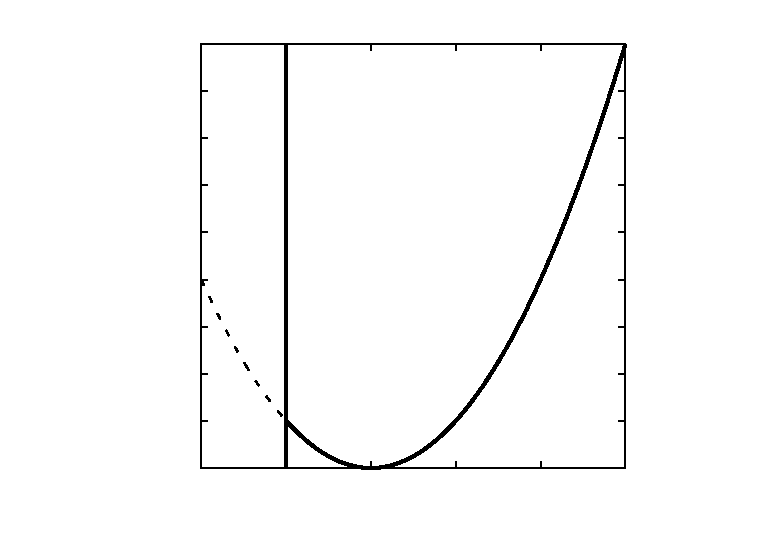
\includegraphics{delta_mass}}%
    \gplfronttext
  \end{picture}%
\endgroup

\caption{Scaling dimensions $\Delta$ corresponding to a given bulk mass for a scalar field, alongside the unitarity bound $\Delta\geq 1$.}
\end{figure}

where only solutions $\Delta \geq 1$ are to be considered\footnote{The bound $\Delta \geq 1$ for a 4D CFT is the unitarity bound for free scalar fields.}. It would seem as if the smallest possible dimension of a boundary operator is $4$, however one should take into account the fact that the hyperbolic curvature of $AdS$ produces an effective confining potential that allows particles with $m^2 < 0$ to be stable. It can be shown that the Breitenlohner-Freedman bound holds for stable scalar fields

\begin{equation}
	m^2 R^2 \geq - 4
	\label{}
\end{equation}

so that it is possible to reach down to the unitarity limit at $\Delta = 1$.\\

This was for scalar fields. Higher-spin fields will be dual to operators of the same spin on the boundary and the $m-\Delta$ equation will be modified. For example, $(\frac{1}{2},\frac{1}{2})$ vectors will have

\begin{equation}
	R^2 m^2 = (\Delta-1)(\Delta-3)
	\label{}
\end{equation}

while $(1,1)$ symmetric tensor will instead have the same equation as scalars:

\begin{equation}
	R^2 m^2 = \Delta (\Delta-4)
	\label{}
\end{equation}

The relevance of this is that the operators coupled to massless spin $1$ or $2$ bosons must be conserved currents by gauge invariance, and so the operators dual to a massless bulk photon or graviton are a conserved vector current and the stress-energy tensor, respectively. The anomalous dimensions of these conserved currents must vanish, and indeed $\Delta_J = 3$ and $\Delta_T = 4$ are canonical.

\section{AdS/CFT over a cone}

As seen above, the original motivation for the AdS/CFT conjecture is the identification of a system of $N$ coincident D3-branes in a $\mathbb{M}^{10}$ Minkowski background and the corresponding 3-brane supergravity solution. In an appropriate low-energy limit a system of closed IIB strings on flat spacetime decouples in both pictures, suggesting it should be conjectured that the remaining parts are equivalent. These are respectively $\mathcal{N}=4$, $SU(N)$ SYM on $\mathbb{M}^4$ and IIB strings on $AdS_5 \times S_5$.\\

We repeat this reasoning, but in the more interesting case where the background for the D3-branes is generalized as $\mathbb{M}^4 \times X_6$, where $X_6$ is a cone over a base 5-manifold $Y_5$. We anticipate the bulk dual in this case is IIB strings over $AdS_5 \times Y_5$. By $X_6$ being a cone over $Y_5$ it is meant that the metric on it is

\begin{equation}
	ds^2_6 = dr^2 + r^2 ds_5^2 \label{conemetric}
\end{equation}

where of course $ds_5^2$ is the metric on $Y_5$. If $Y_5 = \mathbb{S}^5$ with the unit round metric then the cone is $X_6 = \mathbb{R}^6$ and one returns to the flat case.\\

For this to be a string background, $X_6$ should be Ricci-flat. This is equivalent to $Y_5$ being Einstein of positive curvature. $ds_6^2$ is conformally equivalent to the canonical metric on a cylinder over $Y_5$, as evidenced by the reparametrization $\phi = \ln r$:

\begin{equation}
	ds_6^2 = e^{2\phi} \left( d\phi^2 + ds_5^2 \right)
\end{equation}

Recalling the transformation law of the Ricci tensor in $n$ dimensions under conformal rescalings:

\begin{equation}
	R_{ij}' = R_{ij} - (n-2)\left( \nabla_i \partial_j \phi - \partial_i \phi \partial_j \phi \right) + \left( \nabla^2 \phi - (n-2) \nabla_k \phi \nabla^k \phi \right) g_{ij}
\end{equation}

And noting that for the cylinder the restriction of $R_{ij}$ to $Y_5$ indices gives $Y_5$'s own Ricci tensor $R_{ij}^{(5)}$, we obtain

\begin{equation}
	R^{(5)}_{ij} = 4 g_{ij}^{(5)}
\end{equation}

proving $Y_5$ is Einstein.\\

We are also interested in $X_6$ being Calabi-Yau, that is being K\"ahler with holonomy $\subset SU(3)$. We define $Y_5$ to be Sasaki-Einstein iff the corresponding cone is Calabi-Yau. The complex structure on the cone induces a vector field on the base, the Reeb vector:%nota: da scholarpedia

\begin{equation}
	\xi := J (r \partial_r)
\end{equation}

where $J$ is the complex structure on the cone and $\xi$ is to be thought of as restricted to, say, ${r=1} \cong Y_5$; this is a Killing vector on the base, inducing a 1-dimensional foliation. The dual form, $\theta = g_{ij} \xi^i dx^j$, is a contact form for the base, contact meaning the 2-form on the cone

\begin{equation}
	\omega = t^2 d\theta + t dt \wedge \theta
\end{equation}

is symplectic. This is of course the symplectic form associated to the hermitian structure.\\

After placing 3-branes in this $X_6 \times \mathbb{R}^4$ background, parallel to the Minkowski, the resulting geometry from their backreaction is:

\begin{equation}
ds^2 = H^{-1/2}(r,y) \, dx\cdot dx + H^{1/2}(r,y) \, ds_6^2
\end{equation}
\cmmnt{già fatto! ref ref ref}
Where $x^{0,\ldots,3}$ are coordinates parallel to the brane stack, $dx\cdot dx = -(dx^0)^2 + (dx^i)^2$, $r$ is the radial coordinate and the remaining $y^{1,\ldots,5}$ parametrize the cone's base $Y_5$. This is a simple generalization of the well-known black 3-brane solution by substitution of $\mathbb{S}^5$ with $Y_5$.\\

Ricci-flatness implies the function $H$ is harmonic: $\nabla H(r) = 0$. The linearity of this equation arises from the fact that D-branes are BPS states, corresponding in the gravitational picture to extremal p-branes; these notably do not interact mutually.\\

If the branes are coincident, the corresponding harmonic potential is

\begin{align}
 H(r) = 1 + \frac{R^4}{r^4} && R^4 = 4 \pi g_s N \alpha'^2 
\end{align}

The near-horizon limit ($r\rightarrow 0$) in that case can be read immediately:

\begin{equation}
ds^2 = \frac{ dx \cdot dx + dz^2}{z^2} + ds_5^2
\end{equation}

where $z := 1/r$; this is evidently the product metric on $AdS_5 \times Y_5$, where of $AdS_5$ we're only considering the Poincaré patch. \\

We note that the introduction of a conical singularity results in reduced supersymmetry. Unbroken SUSY generators are identified from the Killing spinor equation:

\begin{equation}
	\left(\partial_\mu + \frac{1}{4} \omega_{\mu\alpha\beta} \Gamma^{\alpha\beta} \right) \eta = 0
\end{equation}

Explicitly for the cone metric \ref{conemetric}:

\begin{equation}
	\left(\partial_i + \frac{1}{4} \omega_{ijk} \Gamma^{jk} + \frac{1}{2} \Gamma^r_i \right) \eta = 0
\end{equation}

this is, as expected, coincident with the ($Y_5$ sector of) Killing spinor equation for the backreacted $AdS_5 \times Y_5$ geometry, including also the effect of $F_5$. This is to show there is a match between the unbroken SUSYs in the bulk theory and in the boundary.\\

If the cone is of holonomy $SU(n)$, this will result in a reduction of supersymmetries by a factor of $2^{1-n}$ with respect to $\mathbb{M}^{10}$ Minkowski. In particular, if $X_6$ is Calabi-Yau, then the $32 = 16 \times 2$ fermionic generators of IIB SUGRA are reduced to $32 \times 2^{-2} = 8$, which means the SCFT in $4D$ has $\mathcal{N}=1$ (in contrast to the usual SUSY algebra, the $\mathcal{N}=1$ $4D$ superconformal group has both $4$ supertranslations and $4$ additional fermionic superconformal generators). If, instead, we were to consider the more restrictive case of manifolds of $SU(2)$ holonomy, there would be $16$ unbroken supersymmetries signaling an $\mathcal{N}=2$ dual SCFT.

%\section{The Klebanov-Witten model}
%
%\cmmnt{???}
%
%A well-known specific example of SCFT holographically dual to D-branes in a Calabi-Yau cone has been introduced in \cite{KW_SCFT}. In this case the base of the cone is the manifold $T^{1,1} = (SU(2)\times SU(2))/U(1)$, where $U(1) \subset SU(2)_L\times SU(2)_R$ is generated by $\sigma^3_L + \sigma^3_R$.\\
%
%We give a characterization of the cone $X_6$ over $T^{1,1}$ as a submanifold of $\mathbb{C}^4 \ni (A^1,A^2,B^1,B^2)$ given by
%
%\begin{equation}
%	|A^1|^2 + |A^2|^2 - |B^3|^2 - |B^4|^2 = 0
%\end{equation}
%
%quotiented by $U(1)$ acting on $A^i$ with charge $1$ and $B^i$ with charge $-1$. This makes the $SU(2)\times SU(2) \approx SO(4)$ symmetry manifest with the two copies of $SU(2)$ acting respectively only on $A^i$ and $B^i$.\\
%
%
%The holographic dual theory to a stack of $N$ D3-brane moving in the background given by $\mathbb{R}^4$ times the cone over $T^{1,1}$ is found to be an $\mathcal{N}=1$ superconformal quiver gauge theory with gauge group $SU(N)\times SU(N)$, with chiral superfields $A^i$, $B^i$ ($i=1,2$) transforming respectively in the bifundamentals $(\mathbf{N},\mathbf{\bar N})$, $(\mathbf{\bar N},\mathbf{N})$. The $SU(2)\times SU(2)$ isometry in the bulk is here implemented as a "flavour" global symmetry acting separately on $A^i$ and $B^i$. Moreover, the diagonal $U(1)$ reappears as a baryonic symmetry where again $A^i$ has charge $1$ and $B^i$ charge $-1$.\\
%
%
%\cmmnt{relazione fra i campi della CFT e la posizione delle D-brane, moduli space mesonico e totale, un po' di più sul KW}
%
